\pagestyle{fancy}
\fancyhf{}
\rhead{Simulation}
\lhead{Chapter 4}
\lfoot{\footnotesize{MES COE, B.E. COMPUTER YEAR 2021-22}}
\rfoot{\thepage}


\chapter{Simulation}

In the presence of two interfering signals and noise,both amplitude and phase comparison between desired signal and estimated output,beam patterns of the smart antennas and learning characteristics of the above mentioned algorithms are compared and analyzed. In the simulation,the smart antenna of 8 elements has been taken.The smart antenna algorithms compute the antenna weights for all eight antenna elements so that the signal-to-noise-and interference ratio (SINR) becomes optimum\cite{ADR3}.



\section{LMS}
\vspace{-0.5cm}
\begin{figure}[!h]
\hspace{-2.9cm}
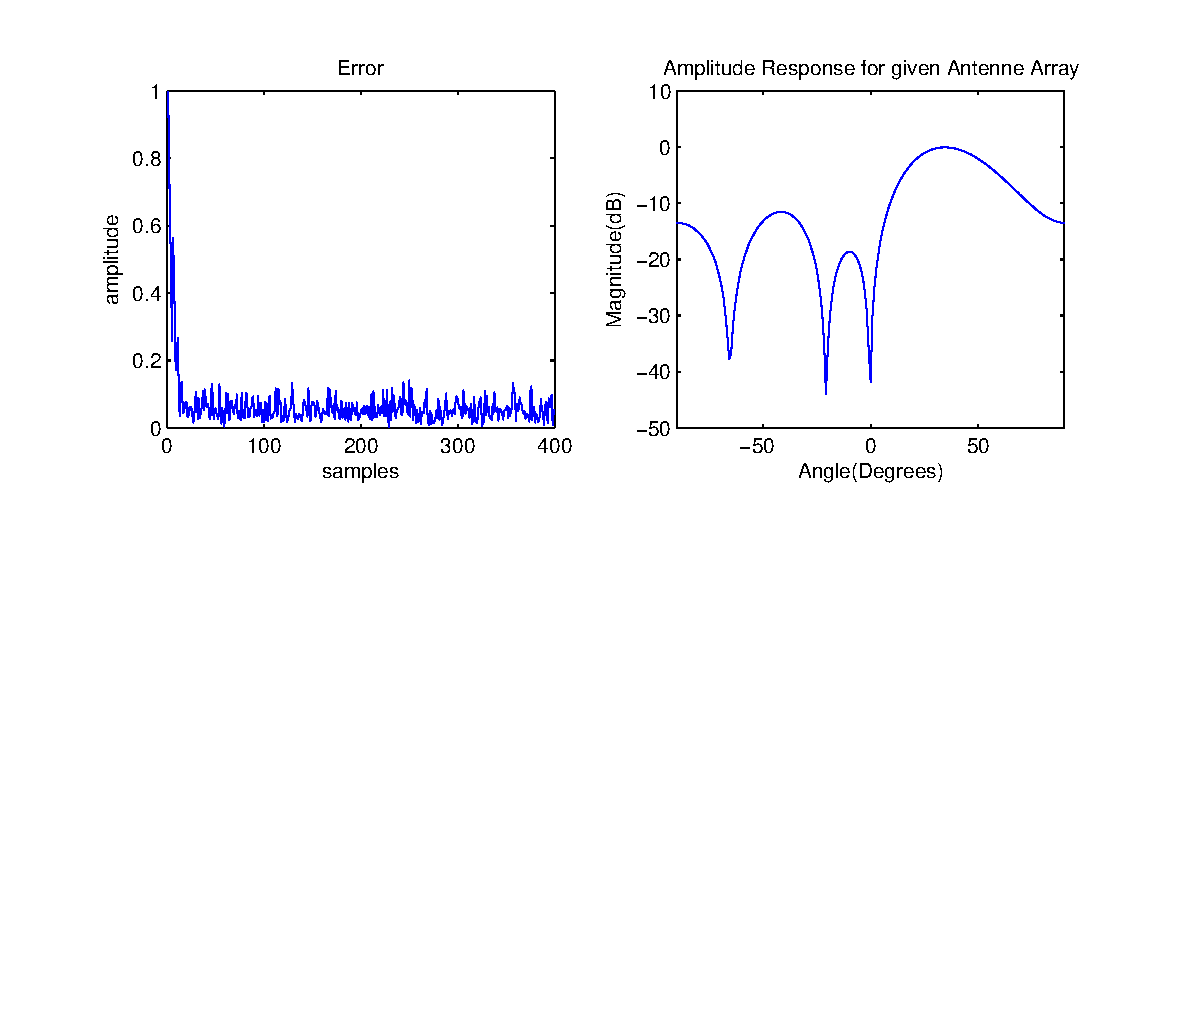
\includegraphics[scale=1.1]{lms1.eps}
\vspace{-10cm}
{\bf{\caption{Error and amplitude response plots for LMS}}}
\end{figure}



